%%%%% DOCUMENT CLASS
\documentclass[12pt]{article}

%%%%% IMPORTING PACKAGES
\usepackage{geometry} % page format
\usepackage{setspace} % page format
\usepackage{amsmath, amsthm, amssymb} % math stuff
\usepackage{mathtools} % math stuff
\usepackage{empheq} % math stuff
\usepackage{cancel} % math stuff
\usepackage{tikz} % for making figures
\usepackage{graphicx} % for figures
\usepackage{placeins} % for figure placement
\usepackage{caption, subcaption} % for figures
\usepackage{enumitem} % for lists
\usepackage{matlab-prettifier} % for MATLAB code
\usepackage{verbatim} % for pasting .txt files
\usepackage{array} % table stuff
\usepackage{threeparttable} % table stuff
\usepackage{tabularx} % table stuff
\usepackage{multirow} % table stuff
\usepackage{colortbl} % table stuff
\usepackage{booktabs} % table stuff
\usepackage{pdfpages} % for importing pdfs
\usepackage{hyperref} % for hyperlinks
\usepackage{titletoc} % for TOC
\usepackage[table,dvipsnames]{xcolor} % for text coloring
\usepackage[backend=biber,sorting=none,style=numeric-comp]{biblatex} % for references
\usepackage{lipsum} % for filler
\usepackage{comment} % for comments

%%%%% CONFIGURING PACKAGE SETTINGS
\geometry{letterpaper,left=1in,top=1in,right=1in,bottom=1in}
\singlespacing
\graphicspath{ {./Figures/} }
\allowdisplaybreaks[1]
\hypersetup{colorlinks=true, linkcolor=red, filecolor=magenta, urlcolor=blue}
\addbibresource{bib.bib}

%%%%% CREATING CUSTOM COMMANDS
\newcommand{\mainmatter}{\clearpage\setcounter{page}{1}\pagenumbering{arabic}}
\newcommand{\appendixpagenumbering}{\clearpage\pagenumbering{arabic}\renewcommand{\thepage}{A-\arabic{page}}}
\newcommand\innercontentsname[1]{%
Contents for section~\ref{#1}}
\newcolumntype{P}[1]{>{\centering\arraybackslash}p{#1}}
\newcolumntype{M}[1]{>{\centering\arraybackslash}m{#1}}
\newcolumntype{R}[1]{>{\raggedleft\arraybackslash}m{#1}}
\renewcommand\tabularxcolumn[1]{m{#1}}

% whatever math operators we need
\DeclareMathOperator{\sgn}{sgn}
\DeclareMathOperator{\acos}{acos}
\DeclareMathOperator{\atantwo}{atan2}
\DeclareMathOperator{\diag}{diag}
\DeclareMathOperator{\spec}{spec}

%%%%% DOCUMENT
\begin{document}

%%%%% TITLE PAGE
\begin{titlepage}
\begin{center}
    \vspace*{\fill}
    {\Huge MAE 5810 Homework 2 Report}\\
    % {\large Midterm Project Report}

    \vspace{4\baselineskip}
    Daniel Whitman\\
    Robot Perception (MAE 5810)\\
    10/02/2026
\end{center}

% \vspace{4\baselineskip}
% \noindent \textbf{ABSTRACT:}
% \noindent Words (maybe we move this to first page? Not really clear what she wants) \lipsum[1]

\vspace*{\fill}
\end{titlepage}

%%%%% ACTUAL REPORT
\mainmatter
\section{INTRODUCTION}\label{sec:intro}
The objective of this assignment is to gain familiarity with the creation, structure learning, and parameter learning of Bayesian networks (BNs) through gathered data. Once properly constructed, these models are remarkably powerful for inferring results from observed data, and can act as a flexible tool in robotic perception applications. The usage that this homework assignment is derived from is in using a BN to predict the propagation loss (PL) or range (R) of an underwater sonar acoustic measurement given different environmental conditions and sensor observations \cite{Cai2007BNMoAS}.

In acoustic sensor measurements, which are observed due to pressure variations in the medium against the sensor, the following acoustic propagation model based on a three-dimensional, time-dependent wave equation \cite{Etter1996UAM} is used:
\begin{align}\label{eqn:acoustic}
    \frac{\partial^2 p}{\partial r^2}+\frac1r\frac{\partial p}{\partial r}+\frac{\partial^2p}{\partial z^2}+k^2(z)p&=0
\end{align}
where $p$ is acoustic field pressure, $r$ is the horizontal distance from a point source, $z$ is the depth below the ocean surface, $k=2\pi f/c=2\pi/\lambda$ is the wave number, $\lambda$ is the wavelength, $f=\omega/(2\pi)$, and
$\omega$ is the source frequency.

From this, the propagation loss (PL) is defined, in decibels ($dB$), as
\begin{align}\label{eqn:PL}
    PL&=-20\log|p|
\end{align}
and, in the far-field assumption of the acoustic modeling \cite{Etter1996UAM} is a function of the following variables:
\begin{enumerate}
    \item Range ($R$)
    \item Depth ($Z$)
    \item Sea Floor ($SF$)
    \item Bottom Density ($BD$)
    \item Bottom Sound Speed ($V$)
    \item Source Frequency ($F$)
\end{enumerate}

In relation to the BN, these six variables correspond to the inputs to be observed and the propagation loss corresponds to the final output of the system. In the network model, each variable is represented as a node, and the connections between then are represented as the edges of the graph.

\section{DESCRIPTION OF DATA}\label{sec:data}
For this homework, the provided dataset was an simulated from the governing equations in (\ref{eqn:acoustic}) and packaged into a MATLAB \texttt{.mat} file. As the data was simulated, it is complete, meaning that no observation were missed from any of the cases within the set. Table \ref{tab:nodes} provides the resulting instantiations of each of the input variables as well as the output PL, resulting in a total of 40000 data points within the set. Figure \ref{fig:pldist} shows the distribution of PL across all of the data points in the set.

\begin{table}[htb]
    \centering
    \caption{List of Nodes in BN Acoustic Model}
    \label{tab:nodes}
    \begin{tabular}{M{0.4\textwidth}M{0.3\textwidth}M{0.2\textwidth}}
        \toprule
        \textbf{Node} & \textbf{Range} & \textbf{Instantiations}\\
        \midrule
        Range ($m$): $R$ & $100:100:1000$ & 10\\
        Depth ($m$): $Z$ & $50:50:500$ & 10\\
        Sea Floor $SF$: & flat (1), uphill (2), downhill (3), up and down (4) & 4\\
        Bottom Density ($g/cc$): $BD$ & $1.5:0.1:2.4$ & 10\\
        Bottom Sound Speed ($m/s$): $V$ & quadratic experiential function of $BD$ & 10\\
        Source Frequency ($Hz$): $F$ & $10:20:200$ & 10\\
        Propagation Loss ($dB$): $PL$ & discretized in model & 10\\
        \bottomrule
    \end{tabular}
\end{table}

\begin{figure}[htb]
    \centering
    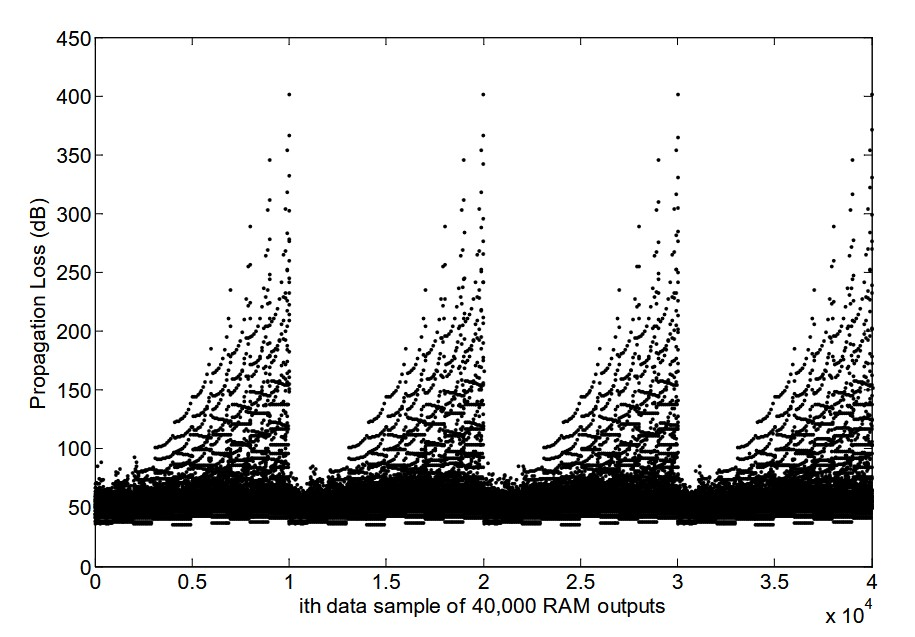
\includegraphics[width=0.7\textwidth]{Figures/PLdist.jpg}
    \captionsetup{justification=centering}
    \caption{Resultant PL across the 40000 data points within the provided dataset}
    \label{fig:pldist}
\end{figure}

\section{CONSTRUCTING THE NETWORK}\label{sec:network}
To construct the BN and perform inference, the Bayes Net Toolbox (BNT) \cite{BNT} was implemented in MATLAB. 

\subsection{PREPROCESSING THE DATA}
To process the data and prepare it for the creation of the BN, first the data was uploaded into the program. Next, the PL data had to be discretized into separate ``bins'' so that the BNT could properly handle the points within its functions. While the toolbox can handle continuous variables, it fails when there are \textit{both} continuous and discrete variables within the set. So, within the set, as the input instantiations were chosen regularly, they are known to be discrete variables, while the PL result from simulation is a continuous real number. To discretize the PL, 10 logarithmically-spaced bins were chosen such that any point within that bin was assigned a single discrete value, regardless of internal spread or variance. The reason that logarithmically-spaced bins were chosen over linearly-spaced bins is that the data in Figure \ref{fig:pldist} is \textit{not} linearly distributed, with more points concentrated near the lower end than the higher end. Therefore, logarithmic spacing allows ``wider'' bins near the top to increase the number of points in them, hopefully giving more weight for structure/parameter learning for these sparse data regions. However, regardless of the bins, discretizing the PL data has the potential to greatly decreases the performance of the BN (as will be discussed later), as the feature size of the PL is massively diminished, but it is a limitation that must be implemented to properly interface with the MATLAB BNT.

Once all the variables were discretized, the data points were randomly shuffled and split into a training set and testing set at ($80\%/20\%$), respectively. Shuffling the data first ensures that the training should not be biased by variable instantiation order within the data set, providing a more generalizable result.

\subsection{DETERMINING THE NETWORK STRUCTURE}
To construct the BN, first the structure of the connection between the nodes had to be learned. To do this, the BNT's ``greedy'' K2-algorithm was implemented (\texttt{learn\_struct\_k2} \cite{BNT}). In this algorithm, initially each node has no parents. Then, parents are added incrementally in a way that such that each addition of a parent is the one that most increases the score of the resulting structure (with the score of a particular BN graph being defined from a Bayesian scoring metric \cite{BNT}). When no parents can increase the score, it moves to the next node and repeats. One caveat of using this method is that the nodes need to be given a prior topological ordering, where parents \textit{must} come before child nodes in the ordering. For our cases, however, this is simple to achieve, as it is known that all the nodes have the potential to become parents for the PL node, so in the ordering, PL is last. In the case that the order is not known, a different search algorithm must be used. Figure \ref{fig:network} gives the final learned structure of the BN for 10 logarithmically-spaced PL bins. As can be seen, from the training data and K2 algorithm only \textbf{three} nodes were found to be parents to the PL loss (node 7). Those nodes are: frequency $F$ (2), depth $Z$ (5), and range $R$ (6). During testing, this was the structure that was always found, regardless of if the discretization bins were set to be linear or logarithmic, and even if the number of bins were increased. The reason for this is most likely due to the poorly-shaped and distributed nature of the data, as through discretizing the PL, \textit{most} of the resulting points will be in the first few bins, and so other such variables (i.e., sea floor $SF$, bottom density $BD$, and bottom sound speed $V$) are ``absorbed'' into the discretization, where their changes do not cause the data to fluctuate greatly enough to ``hop'' bins, thus removing their perceived influence on the PL. This is one of the major downsides for discretizing a continuous variable for the sake of BN training. As previously mentioned, the ``feature space'' of PL is reduced to such a degree that certain variables no longer have an impact, limiting the usefulness of the network for inference to the ``solitary'' nodes.

\begin{figure}[htb]
    \centering
    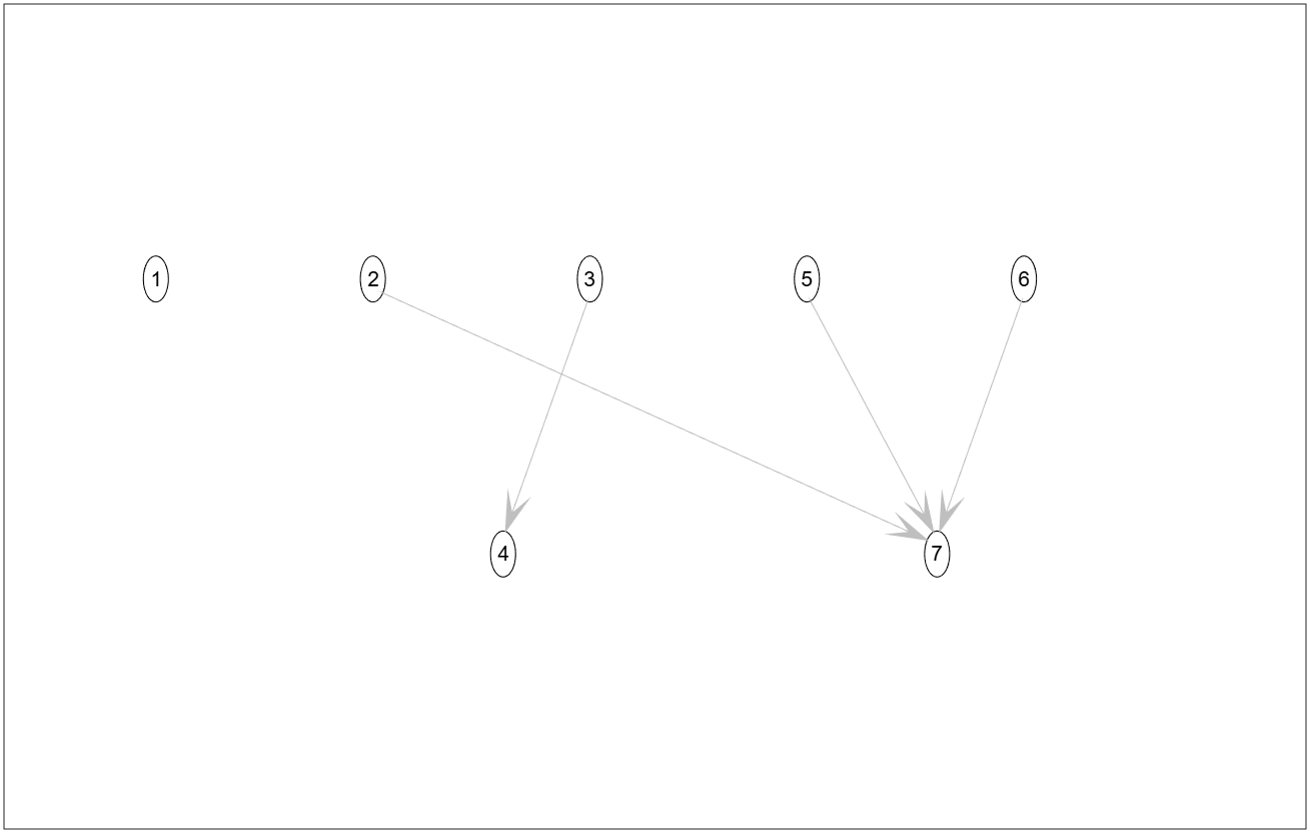
\includegraphics[width=0.6\textwidth]{Figures/Network.png}
    \captionsetup{justification=centering}
    \caption{Resulting BN structure learned for 10 logarithmically-spaced PL bins}
    \label{fig:network}
\end{figure}

\subsection{PARAMETER LEARNING}
Once the network structure is learned from the data, the actual parameters (which are the CPTs corresponding to each node) must be learned from the data. To do this, the BNT's maximum likelihood algorithm ($\hat\Theta=\{\hat\theta_{ijk}\}=\arg\max_{\{\theta_{ijk}\}}\{p(T|S,\Theta)\}$) was implemented (\texttt{learn\_params} \cite{BNT}). In this algorithm, the network was initialized with random CPT parameters, which are then optimized over to find the parameter arguments that maximize the likelihood of recovering the training data $T$ given the structure $S$ and parameters $\Theta$. In relation to the PL (node 7), the resulting CPT is a table that has $10\times10\times10\times10$ entries, which is far too large to include in this right up, but it contains the conditional probabilities of the PL being in ``bin'' $i\in\{1,10\}$ given the discrete value of the range $R$, depth $Z$, and frequency $F$.

\section{RESULTS AND ANALYSIS}\label{sec:results}
Now that the parameters of the BN are learned, it is complete and can be used to perform inferencing.

\subsection{INFERENCING}
For this assignment, the inference that was performed was to predict the PL given the other six variables. Note, in the case of the network in Figure \ref{fig:network}, only three of the variables have any effect on the predicted output, but for completion's sake, all six other variables were instantiated to arrive at a prediction. The evidence that was input into the completed BN were the data points from the \textit{testing} set. They were instantiated by, for each point, creating an inference engine (\texttt{jtree\_inf\_engine} \cite{BNT}), including the \texttt{evidence}, then calculating the ``most probably explanation'' (\texttt{calc\_mpe} \cite{BNT}) given the evidence and engine. This function determines the most-probable discrete outcome of the PL given the observations, rather than providing a probability distribution for the final confidence of the PL in each state. This is the standard method for actually selected a determination from the prediction, as the resulting distribution is not important for the sake of this assignment. Additionally, as the data is \textit{perfect} from simulation (and contains no stochastic noise), the predicted distributions, using the generated BN, were always \textit{singular}, as in perfectly deterministic to a single output value for PL, so they provided no additional information, regardless.

\subsection{SCORING METRICS}
To determine the performance of the BN, four difference metrics were utilized to compare the actual testing PL ($\tilde{PL}$ from the predicted PL ($\bar{PL}$):

\subsubsection{MATCH ACCURACY (MA)}
The case match accuracy ($\hat{MA}$) of any given prediction $\bar{PL}$ compared to the respective true value $\tilde{PL}$ is given as
\begin{align}
    \hat{MA}&=\begin{cases}
        1 & \bar{PL}=\tilde{PL}\\0 & \bar{PL}\neq\tilde{PL}
    \end{cases}
\end{align}

Therefore, for our total inferred PL vector $\underline{\bar{PL}}$ and total testing PL vector $\underline{\tilde{PL}}$, the average match accuracy $MA$ is given as
\begin{align}\label{eqn:MA}
    MA&=\frac1N\sum_{i=1}^N\hat{MA}_i=\frac1N\sum_{i=1}^N\begin{cases}
        1 & \bar{PL}_i=\tilde{PL}_i\\0 & \bar{PL}_i\neq\tilde{PL}_i
    \end{cases}
\end{align}
where $N$ is the total number of testing data points. This method is very straightforward to compute to determine the overall accuracy of the system, however it has disadvantages that it does not consider the ``error distance'' between the prediction and the actual PL, and as a result it cannot be used to determine the confidence interval of the model.

\subsubsection{DISTANCE METRIC (DM)}
The case distance metric ($\hat{DM}$) of any given prediction $\bar{PL}$ compared to the respective true value $\tilde{PL}$ is given as
\begin{align}
    \hat{DM}&=|\bar{PL}-\tilde{PL}|
\end{align}

Therefore, for our total inferred PL vector $\underline{\bar{PL}}$ and total testing PL vector $\underline{\tilde{PL}}$, the average distance metric $DM$ is given as
\begin{align}\label{eqn:DM}
    DM&=\frac1N\sum_{i=1}^N\hat{DM}_i=\frac1N\sum_{i=1}^N|\bar{PL}_i-\tilde{PL}_i|
\end{align}

The advantage of this scoring metric is that the distance between the predicted PL and true PL is captured by the result, and when averaged it provides some measure of the ``mean'' distance between any one prediction and its respective true value. However, this method still does not consider confidence intervals.

One thing to note about computing $DM$ is that the output/inference of the BN is a \textit{discrete} integer giving the bin number that the PL is most likely to reside within. Therefore, to convert this integer value to decibels to match the PL given in (\ref{eqn:PL}), the inferred PL was given as the \textit{central} $dB$ value of its respective bin, allowing for a meaningful $DM$ result.

\subsubsection{DISTANCE EXPECTATION METRIC (DEM)}
The case distance expectation metric ($\hat{DEM}$) of any given prediction $\bar{PL}$ compared to the respective true value $\tilde{PL}$ is given as
\begin{align}
    \hat{DEM}&=|\bar{PL}-E[\tilde{PL}]|
\end{align}
where $E[\tilde{PL}]$ is the expected value of the true PL. We can find the expected value as
\begin{align}
    E[\tilde{PL}]&=\sum_{i=1}^Bp(\tilde{PL}_i=PL_B)PL_B
\end{align}
where $B$ is the number of discrete bins and $PL_B$ is the propagation loss within that bin. To find the actual probability distribution $p(\tilde{PL}=PL_B)$, the frequentest approach was used, where
\begin{align}
    p(\tilde{PL}=PL_B)&=\frac1N\sum_{i=1}^N\begin{cases}
        1 & \tilde{PL}_i=PL_B\\0 & \tilde{PL}_i\neq PL_B
    \end{cases}
\end{align}

Therefore, for our total inferred PL vector $\underline{\bar{PL}}$ and total testing PL vector $\underline{\tilde{PL}}$, the average distance expectation metric $DEM$ is given as
\begin{align}\label{eqn:DEM}
    DEM&=\frac1N\sum_{i=1}^N\hat{DEM}_i=\frac1N\sum_{i=1}^N|\bar{PL}_i-E[\tilde{PL}_i]|
\end{align}

The advantage of this scoring metric over MA and DM is that it now allows for the interpretation of the confidence interval of the results due to the computation of the expected value of PL and the frequentest probability distribution for each bin. As with DM, because the BN only predicts which bin the PL will reside in, the discrete value is also given a corresponding $dB$ value such that the result is physically meaningful.

\subsubsection{NORMALIZED DISCRETE DISTANCE EXPECTATION METRIC}
The case normalized discrete distance expectation metric ($\hat{NDDEM}$) of any given prediction $\bar{PL}$ compared to the respective true value $\tilde{PL}$ is given as
\begin{align}
    \hat{NDDEM}&=|\mathbb B(\bar{PL})-\mathbb B(\tilde{PL})|*ND
\end{align}
where $\mathbb B(\cdot)$ denotes the operation of determining the discrete bin that PL resides in and $ND$ is the neighbor distance
\begin{align}
    ND&=\frac{2(0.5B-1)}{(B-1)(B-2)}=\frac{1}{B-1}
\end{align}
where $B$ is the number of discrete bins.

Therefore, for our total inferred PL vector $\underline{\bar{PL}}$ and total testing PL vector $\underline{\tilde{PL}}$, the average normalized discrete distance expectation metric $NDDEM$ is given as
\begin{align}\label{eqn:NDDEM}
    NDDEM&=\frac1N\sum_{i=1}^N\hat{NDDEM}_i=\frac1N\sum_{i=1}^N|\mathbb B(\bar{PL}_i)-\mathbb B(\tilde{PL}_i)|*ND
\end{align}

An advantage of this scoring metric over the others is that it is developed specifically for discrete variables and that it can be naturally extended for larger and larger discrete sets with minimal computation. However, unlike the others, for continuous variables (such as PL) it requires careful discretization to determine appropriate bins for each of the respective data points.

\subsection{RESULTS}
Table \ref{tab:results} gives the results of BN's performance on the testing data set with respect to each of the four metrics in (\ref{eqn:MA}), (\ref{eqn:DM}), (\ref{eqn:DEM}), and (\ref{eqn:NDDEM}).

\begin{table}[htb]
    \centering
    \caption{List of Nodes in BN Acoustic Model}
    \label{tab:results}
    \begin{tabular}{lr}
        \toprule
        \textbf{Metric} & \textbf{Score}\\
        \midrule
        $MA$ & 0.8671\\
        $DM$ ($dB$) & 2.9924\\
        $DEM$ ($dB$) & 13.1646\\
        $NDDEM$ & 0.0168\\
        \bottomrule
    \end{tabular}
\end{table}

As seen, according to MA, the Bn performed quite well. However, a large reason for this is \textit{because} of the discretization and the ill-prepared dataset. As the majority of the data points were placed into very few bins (mostly bins 1 and 2, with $B=10$), the network only needed to ``learn'' parameters such that for any given evidence, the PL is most likely to be predicted in one of these lower bins to cause high accuracy. Because of this, it is difficult to determine if the model is actually good at predicting proper PL or if the results are simply a function of how congested the data distribution is. This is not just an issue for the MA. Notably, it plagues all of the performance metrics, and while DM and DEM may provide more physically meaningful results, if all points are estimated to have a PL near the lower spread of data, then they too will suffer from falsely-high performance.

Overall, despite the shortcomings of the provided dataset and limitations of the BNT \cite{BNT}, a proper BN was able to be configured, constructed, and training given data and used to infer PL from six other environmental observations, thus demonstrating the powerful impact that this model can have in complex perception challenges.

%%%%% REFERENCES
\clearpage
\printbibliography[title={\textbf{REFERENCES}}]

\end{document}
